\chapter{Supplementary Numerical Details}
\label{app:noise_analysis}

This appendix gives three supporting details for Chapters~\ref{ch:methods} and~\ref{ch:noise_analysis}.  It shows why the two parts of the Transverse-Field Ising Model (TFIM) Hamiltonian do not commute, states finite-shot bounds for VQSE, and fixes the derivative convention for matched-purity paths.  These details make the numerical comparisons reproducible.  They do not add new physical assumptions or conclusions.


\section{Non-commutation of the TFIM Terms}
\label{app:non_commutation}

The global commutator can be checked by looking only at local terms that act on the same qubit.  Operators on different qubits commute, so $Z_{i+1}X_i=X_iZ_{i+1}$.  The remaining calculation reduces to the Pauli relation $[X,Z]=-2iY$ on the shared qubit.
\begin{equation}
    \begin{aligned}
        [X_i, Z_iZ_{i+1}]
         & = X_i (Z_i Z_{i+1}) - (Z_i Z_{i+1}) X_i \\
         & = X_i Z_i Z_{i+1} - Z_i X_i Z_{i+1}     \\
         & = (X_i Z_i - Z_i X_i) Z_{i+1}           \\
         & = [X_i, Z_i] Z_{i+1}                    \\
         & = -2iY_i Z_{i+1}
    \end{aligned}
\end{equation}

The final operator is nonzero, so the full Hamiltonian terms $H_X$ and $H_{ZZ}$ do not commute.  Their time evolutions cannot be separated exactly into independent exponentials.  Section~\ref{sec:trotterization} therefore uses a Trotter decomposition.


\section{Finite-Shot Sampling and Verification Bounds}
\label{appendix:finite_shot_sampling}
% ==============================================================================

VQSE estimates eigenvalues from the empirical bitstring frequencies $f_i/N_{\text{runs}}$.  A finite number of shots therefore introduces sampling noise.

\begin{theorem}[Shot Complexity for Relative Accuracy]
    For one target probability $\tilde{\lambda}_i$, Hoeffding's inequality gives
    \begin{equation}
        \Pr\!\left[
            \frac{|\tilde{\lambda}_i^{\mathrm{est}}-\tilde{\lambda}_i|}{\tilde{\lambda}_i}
            \geq c\right]
        \leq 2\exp\!\left[-2N_{\mathrm{runs}}c^2\tilde{\lambda}_i^2\right]
    \end{equation}
    Applying a union bound to the $m$ retained eigenvalues, a sufficient condition for all relative errors to remain below $c>0$ with probability at least $1-\delta$ is
    \begin{equation}
        N_{\text{runs}}
        \geq\frac{\log(2m/\delta)}{2c^2\tilde{\lambda}_m^2}
        =\mathcal{O}\!\left(\frac{\log(m/\delta)}{c^2\tilde{\lambda}_m^2}\right)
        \label{eq:shot_scaling}
    \end{equation}
    where $\tilde{\lambda}_m$ is the smallest probability among the retained components.
\end{theorem}

The bound is controlled by the smallest retained probability.  Small eigenvalues need many more shots because the required sample size grows as $1/\tilde{\lambda}_m^2$.

\begin{theorem}[Operational Error Verification Bound]
    Define the total eigenvalue error as $\epsilon_\lambda=\sum_{i=1}^m(\lambda_i-\tilde{\lambda}_i)^2$.  Define the eigenvector alignment error as $\epsilon_v=\sum_{i=1}^m\langle\delta_i|\delta_i\rangle$, where $|\delta_i\rangle=(\mathbb{I}-|\tilde{\lambda}_i\rangle\langle\tilde{\lambda}_i|)\rho|\tilde{\lambda}_i\rangle$.  Both errors are bounded by the final cost $C(\boldsymbol{\beta}_{\mathrm{opt}})$.
    \begin{equation}
        \epsilon_\lambda, \, \epsilon_v \le \operatorname{Tr}[\rho^2] - \frac{(E_{m+1} - C(\boldsymbol{\beta}_{\mathrm{opt}}))^2}{\sum_{i=1}^m (E_{m+1} - E_i)^2}
        \label{eq:operational_error_bound}
    \end{equation}
    An optional two-copy verification protocol gives a tighter bound that can be checked on hardware.  It uses $b_m$ sampled bitstrings with $m\leq b_m<2^n$.
    \begin{equation}
        \epsilon_\lambda, \, \epsilon_v \le \operatorname{Tr}[\rho^2] - \sum_{i=1}^{b_m} \tilde{\lambda}_i^2 - \frac{\left(1 - \sum_{i=1}^{b_m} \tilde{\lambda}_i\right)^2}{2^n - b_m}
        \label{eq:verification_bound_2copy}
    \end{equation}
\end{theorem}

The first bound uses the optimized cost to certify both eigenvalues and eigenvectors.  The two-copy version also uses the measured purity and sampled probabilities, so it can give a tighter check after training.




\section{Derivatives for Matched-Purity Paths}
\label{app:matched_purity_derivatives}

In the matched-purity control, the depolarizing probability $P$ and inverse temperature $\beta$ are chosen as functions of the estimated field $h_x$.  The QFI must therefore use the total derivative along each chosen path.

Each derivative has two parts.  One comes from the direct response of the state to $h_x$.  The other comes from changing $P$ or $\beta$ to keep the purity matched.  Leaving out the second part would describe a different path through state space.

For the matched depolarizing family, this derivative is
\begin{equation}
    \frac{\mathrm{d}\rho_{\mathrm{dep},S}}{\mathrm{d}h_x}
    =
    (1-P)\frac{\partial\rho_{\mathrm{G},S}}{\partial h_x}
    -\frac{\mathrm{d}P}{\mathrm{d}h_x}\rho_{\mathrm{G},S}
    +\frac{1}{2^n}\frac{\mathrm{d}P}{\mathrm{d}h_x}\mathbb{I}_S
    \label{eq:matched_depolarizing_derivative}
\end{equation}
For the matched thermal family, it is
\begin{equation}
    \frac{\mathrm{d}\rho_{\mathrm{th},S}}{\mathrm{d}h_x}
    =
    \operatorname{Tr}_E\!\left[
        \frac{\partial\rho_{\mathrm{th},N}}{\partial h_x}
        +\frac{\partial\rho_{\mathrm{th},N}}{\partial\beta}
        \frac{\mathrm{d}\beta}{\mathrm{d}h_x}
        \right]
    \label{eq:matched_thermal_derivative}
\end{equation}

The matched-purity construction therefore compares chosen parameterized state paths.  It is not a fixed-channel experiment.  The full-to-local QFI inequalities in Chapter~\ref{ch:noise_analysis} provide a direct consistency check for these calculations.


\section{Graphical Calculus for Quantum Channels}
\label{app:noise_graphical_calculus}

The diagrams in Chapter~\ref{ch:noise_analysis} provide visual bookkeeping for quantum channels.  A wire represents a system index.  Joining two wires means that the corresponding indices are contracted.  Closing an output wire means that the system is traced out.  A box represents a state, an operator, or a channel, as indicated by its label.  The diagrams follow the tensor-network notation of Ref.~\cite{wood2015graphical}.  Reference~\cite{picturing_quantum_processes_2017} uses a related process-box notation.

Figure~\ref{fig:diagram_extra_equivalence} compares the two styles.  Their shapes and wire directions differ, but they describe the same channel action.  The equations remain the definition of each map.  This is important for the Choi representation because bending an input wire depends on the chosen transpose convention.

\begin{figure}[htbp]
    \centering
    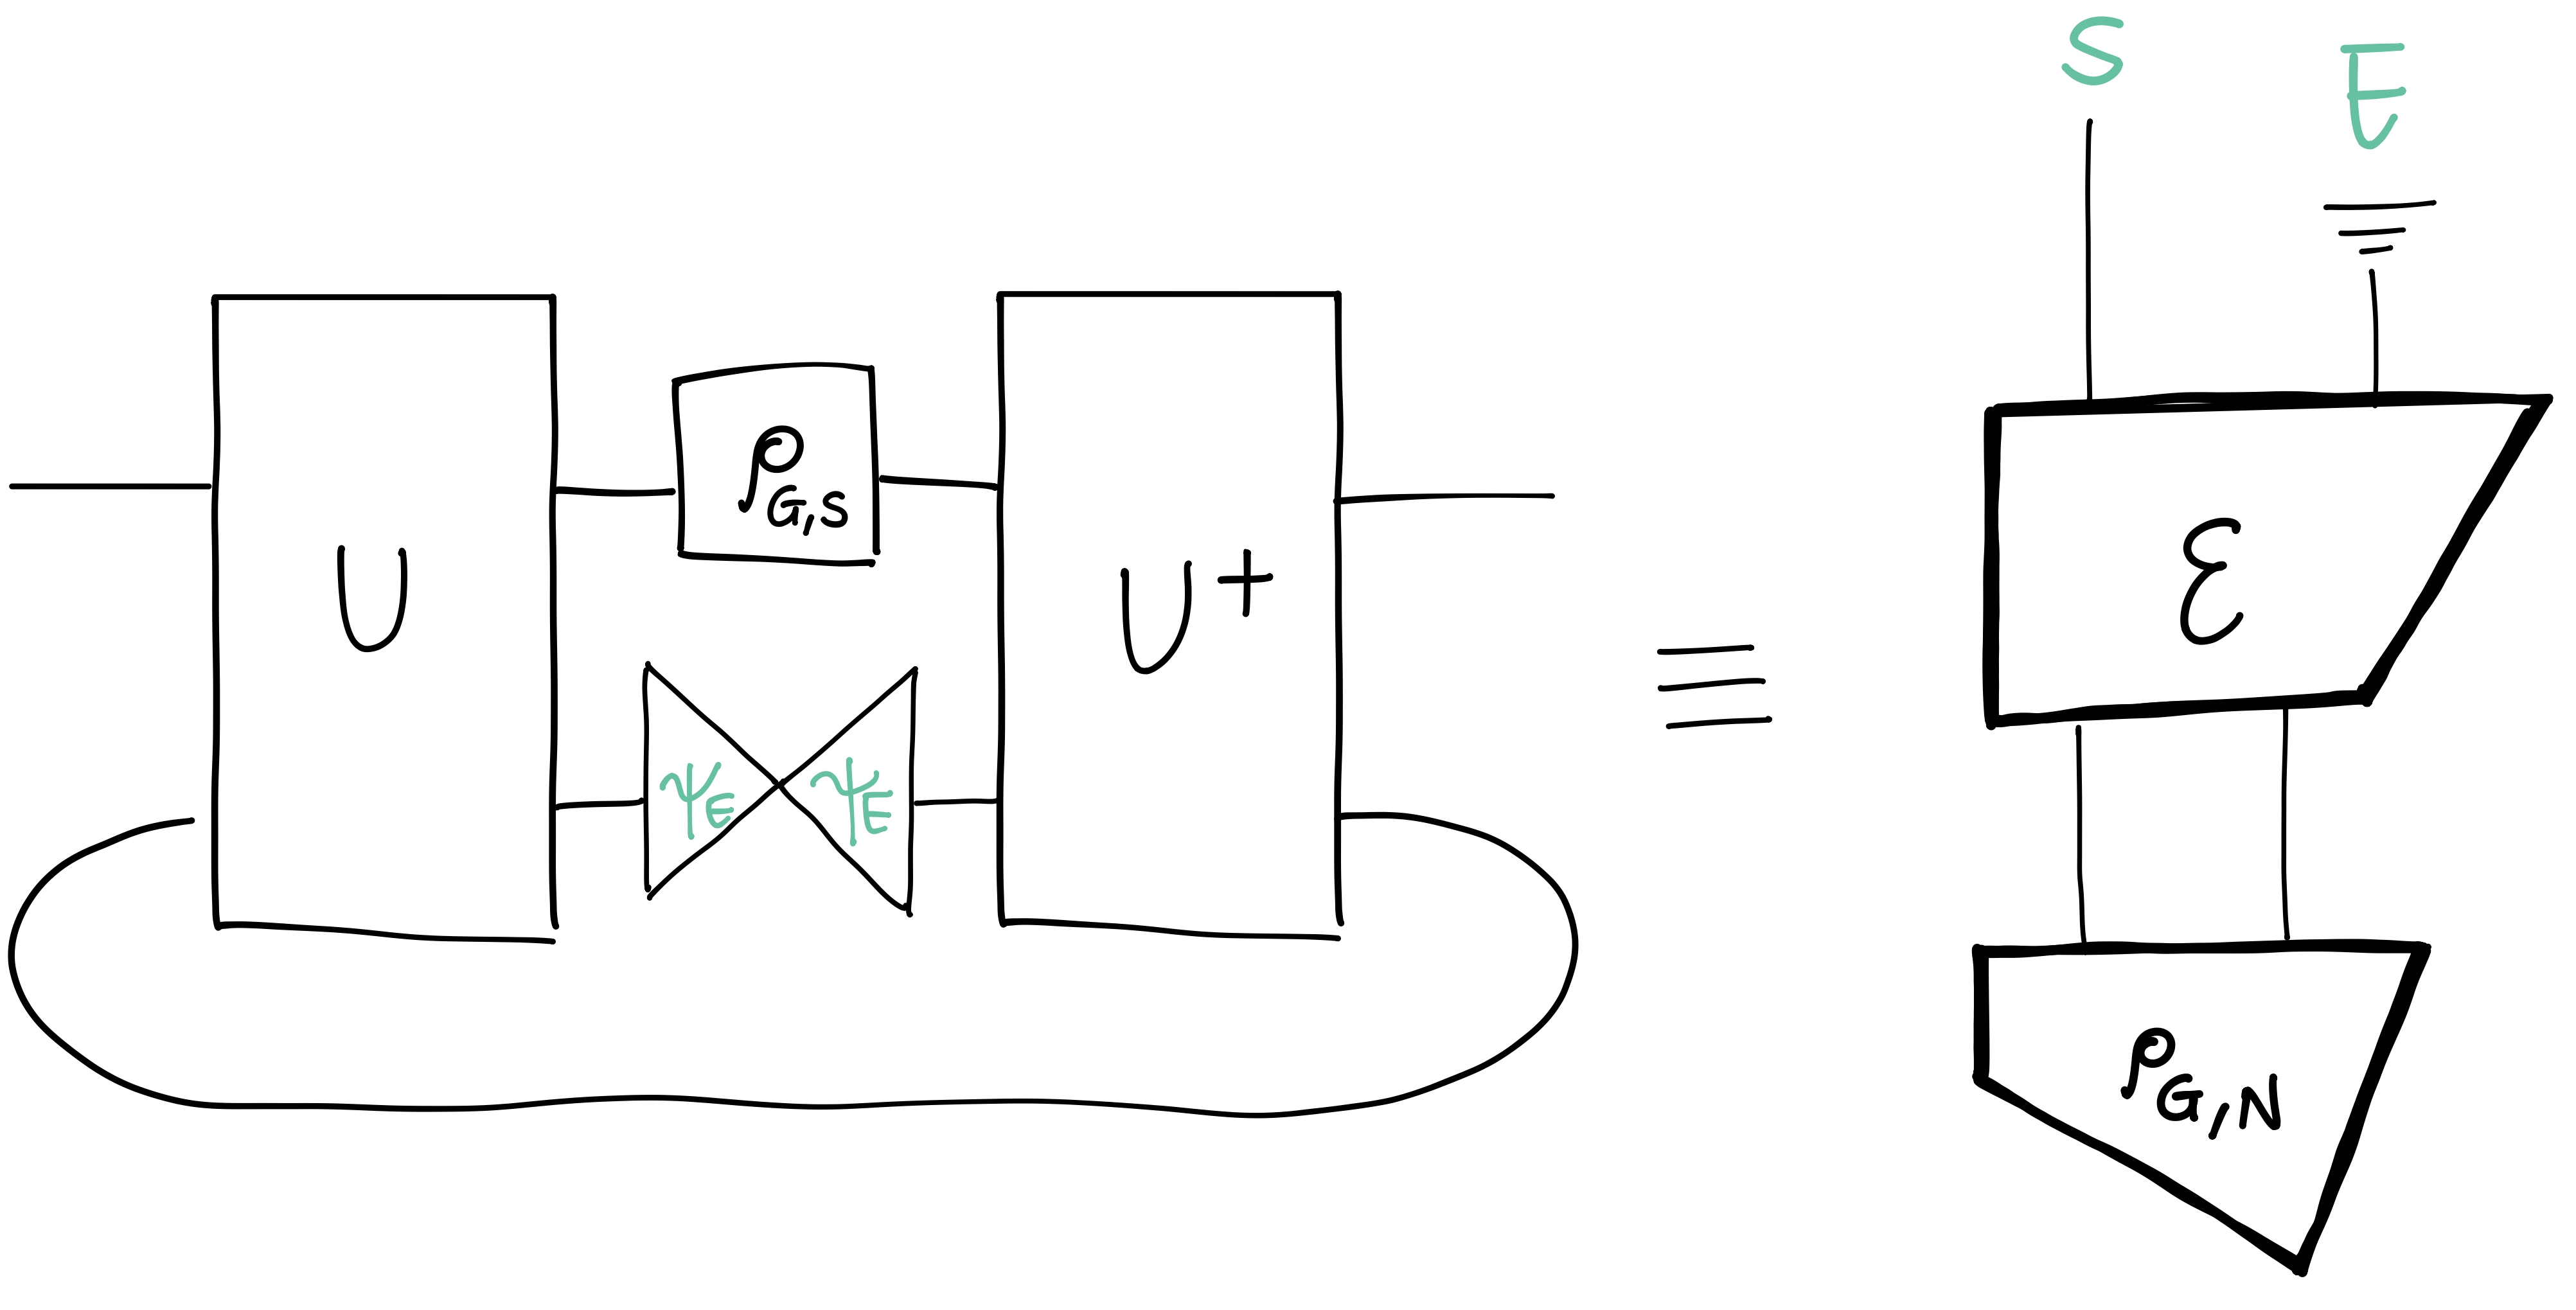
\includegraphics[width=0.7\textwidth]{figures/diagrams/diagram_extra_equivalence.jpg}
    \caption{Two graphical notations for the same channel action.  The tensor-network form from Ref.~\cite{wood2015graphical} is shown on the left.  The process-box form used in Ref.~\cite{picturing_quantum_processes_2017} is shown on the right.  In both cases, closing the environment output represents a trace.}
    \label{fig:diagram_extra_equivalence}
\end{figure}

A Stinespring representation introduces an auxiliary environment $A$ in a fixed state $|\psi_A\rangle$.  A unitary $U$ acts on the input and this environment.  The environment is then traced out.  Choosing an orthonormal basis $\{|i\rangle_A\}$ gives the Kraus operators $K_i={}_A\langle i|U|\psi_A\rangle_A$ and the equivalent expressions
\begin{equation}
    \mathcal{E}(\rho)
    =\operatorname{Tr}_A\!\left[
        U(\rho\otimes|\psi_A\rangle\langle\psi_A|)U^\dagger
        \right]
    =\sum_i K_i\rho K_i^\dagger
    \label{eq:noise_graphical_stinespring_kraus}
\end{equation}
The closed environment wire in Figure~\ref{fig:diagram_stinespring_to_kraus_extended_proof} represents the sum over $i$.  The environment used for this dilation is a mathematical part of the channel representation.  It is not automatically the physical subsystem $E$ discarded in the TFIM calculation.

\begin{figure}[htbp]
    \centering
    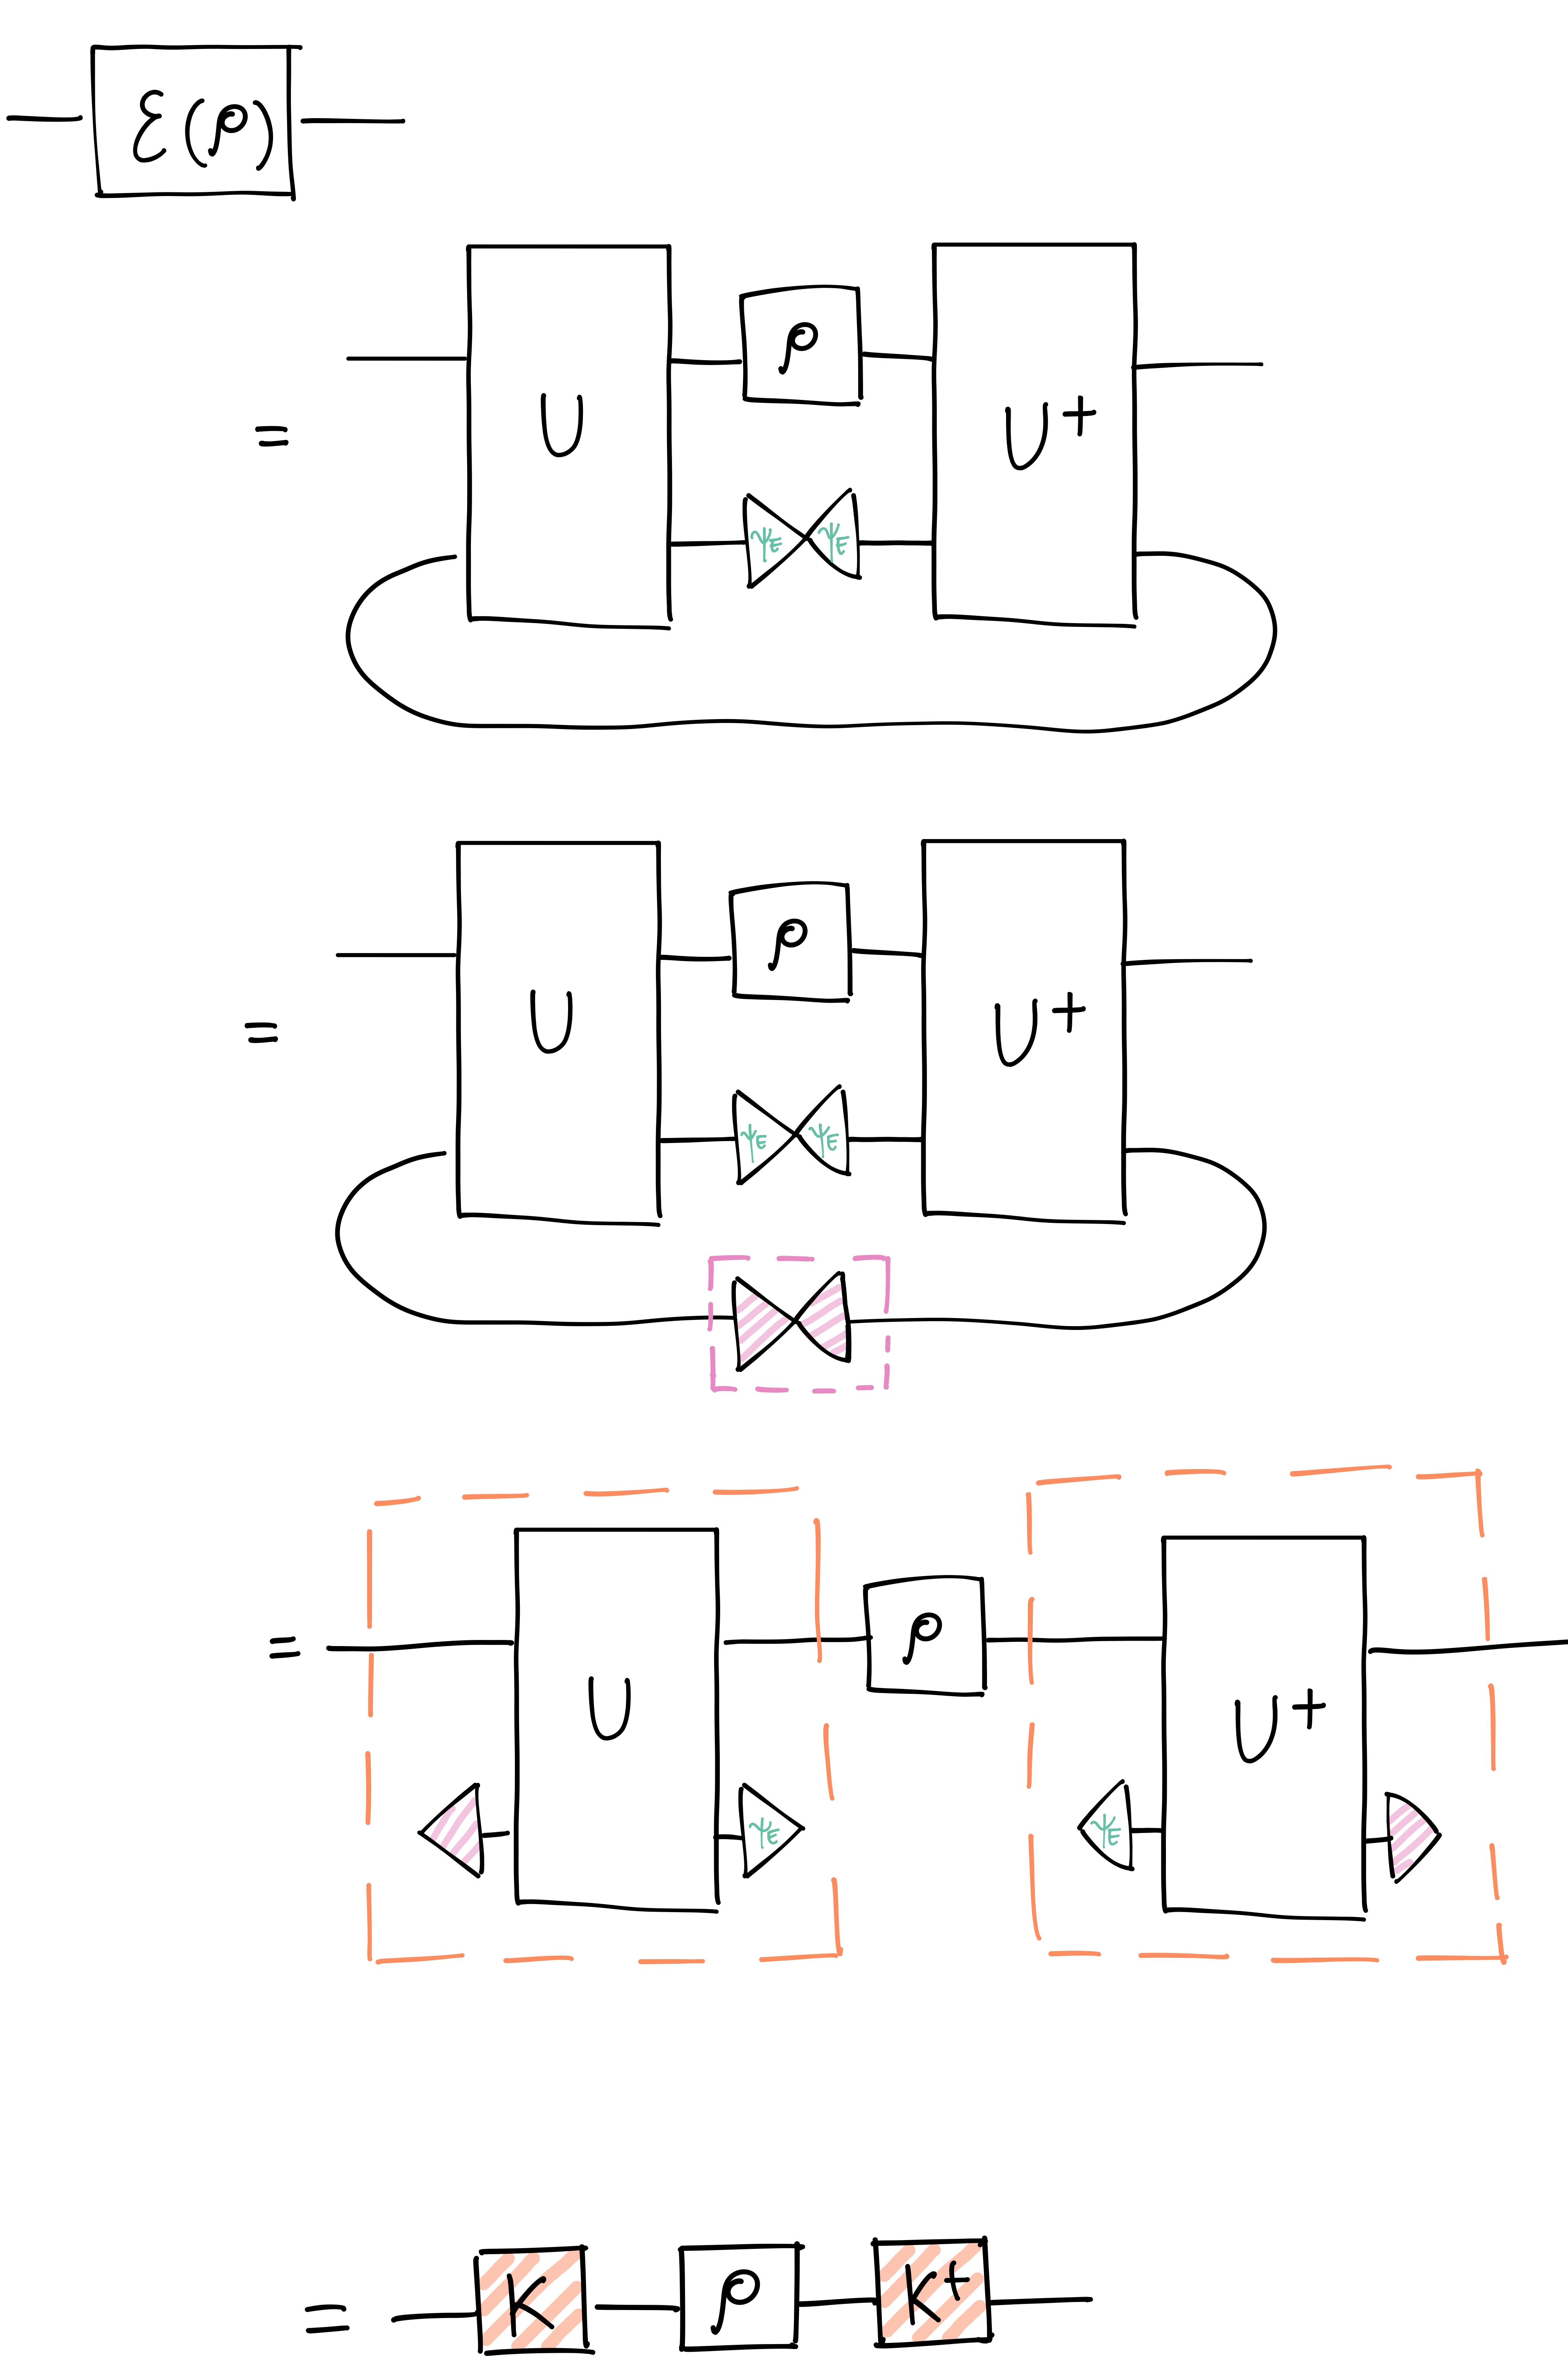
\includegraphics[width=0.7\textwidth]{figures/diagrams/diagram_stinespring_to_kraus_extended_proof.jpg}
    \caption{Graphical reduction from Stinespring form to Kraus form.  The first line applies $U$ and $U^\dagger$ around the input state and closes the environment wire.  Inserting an environment basis resolves this closed wire into Kraus factors.  Grouping the remaining contractions gives $\sum_iK_i\rho K_i^\dagger$, as in Eq.~\eqref{eq:noise_graphical_stinespring_kraus}.}
    \label{fig:diagram_stinespring_to_kraus_extended_proof}
\end{figure}

The Choi matrix is another representation of the same channel.  It contains the channel information in one operator, but it is not the channel map itself.  With the column Choi convention used in this Thesis, its action on $\rho$ is fixed by Eq.~\eqref{eq:choi_channel_action}.  The transpose in that equation is represented graphically by bending the input wire before contracting it with the Choi tensor.  Decomposing the Choi matrix into Kraus factors then gives the same operator-sum expression as Eq.~\eqref{eq:noise_graphical_stinespring_kraus}.

\begin{figure}[htbp]
    \centering
    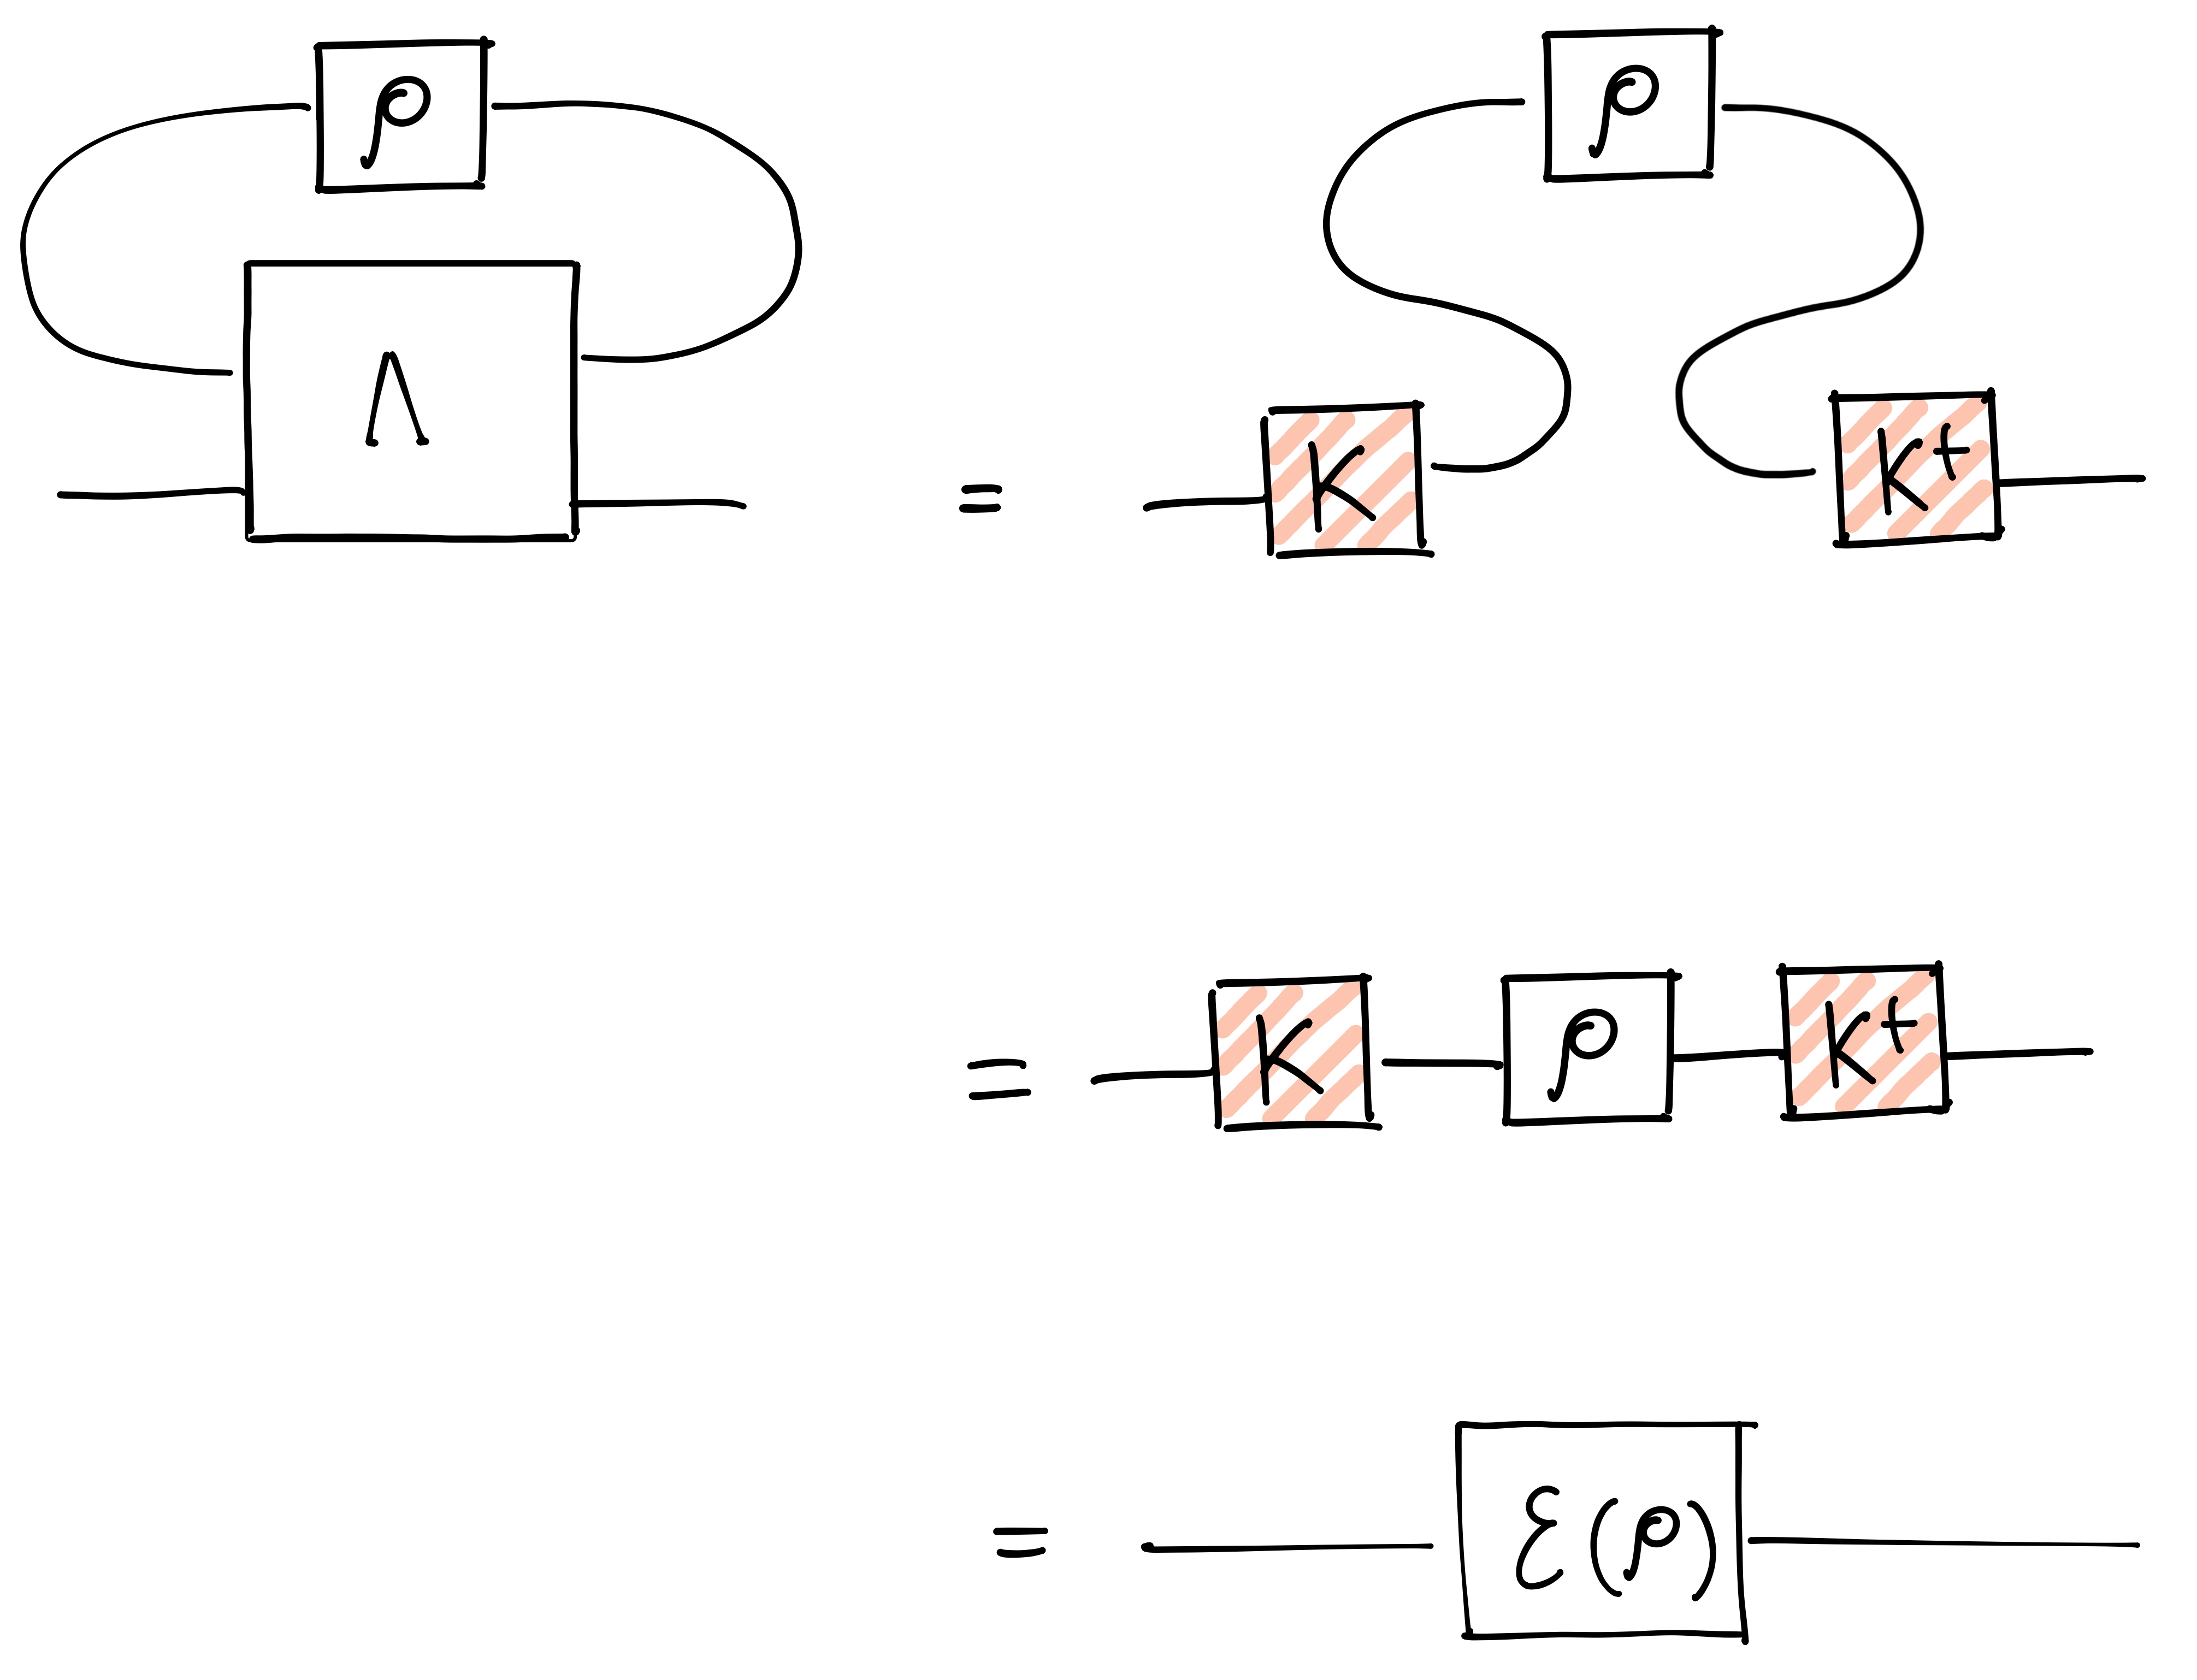
\includegraphics[width=0.7\textwidth]{figures/diagrams/diagram_Choi_to_kraus_extended_proof.jpg}
    \caption{Graphical relation between Choi and Kraus representations.  The input density operator is contracted with the Choi tensor using the convention of Eq.~\eqref{eq:choi_channel_action}.  Factoring the Choi tensor and regrouping its contractions gives the Kraus form.  The closed wire denotes the implicit sum over the Kraus index.}
    \label{fig:diagram_Choi_to_kraus_extended_proof}
\end{figure}
